% https://tex.stackexchange.com/a/299454/173708
% takes 40 seconds to compile
\documentclass[tikz,margin=10pt]{standalone}

\tikzset{pics/gear/.style n args={3}{
    code={
        \def\modu{#1}
        \def\Zb{#2}
        \def\AngleA{#3}

        \pgfmathsetmacro{\Rpr}{\Zb*\modu/2}
        \pgfmathsetmacro{\Rb}{\Rpr*cos(\AngleA)}
        \pgfmathsetmacro{\Rt}{\Rpr+\modu}
        \pgfmathsetmacro{\Rp}{\Rpr-1.25*\modu}
        \pgfmathsetmacro{\AngleT}{pi/180*acos(\Rb/\Rt)}
        \pgfmathsetmacro{\AnglePr}{pi/180*acos(\Rb/\Rpr)}
        \pgfmathsetmacro{\demiAngle}{180/\Zb}
        \pgfmathsetmacro{\Angledecal}{(\demiAngle-2*\AnglePr)/2}

        \path[pic actions] foreach \zz in{1,...,\Zb}{
            \ifnum\zz=1
                % don't use a lineto in the first iteration
                (\zz/\Zb*360-\Angledecal:\Rp)
            \else
                -- (\zz/\Zb*360-\Angledecal:\Rp)
            \fi
            to[bend right=\demiAngle]
            (\zz/\Zb*360+\Angledecal:\Rp)
            --
            plot[domain=-0:\AngleT,smooth,variable=\t]
                ({{180/pi*(-\t+tan(180/pi*\t)) +\zz/\Zb*360+\Angledecal}:\Rb/cos(180/pi*\t)})
            %
            to[bend right=\demiAngle]
                ({{180/pi*(\AngleT+tan(180/pi*-\AngleT)) +(\zz+1)/\Zb*360-\Angledecal}:
                \Rb/cos(180/pi*-\AngleT)})
            --
            plot[domain=-\AngleT:-0,smooth,variable=\t]
            ({{180/pi*(-\t+tan(180/pi*\t)) +(\zz+1)/\Zb*360-\Angledecal}:\Rb/cos(180/pi*\t)})
        } -- cycle;
    }
}}

\begin{document}
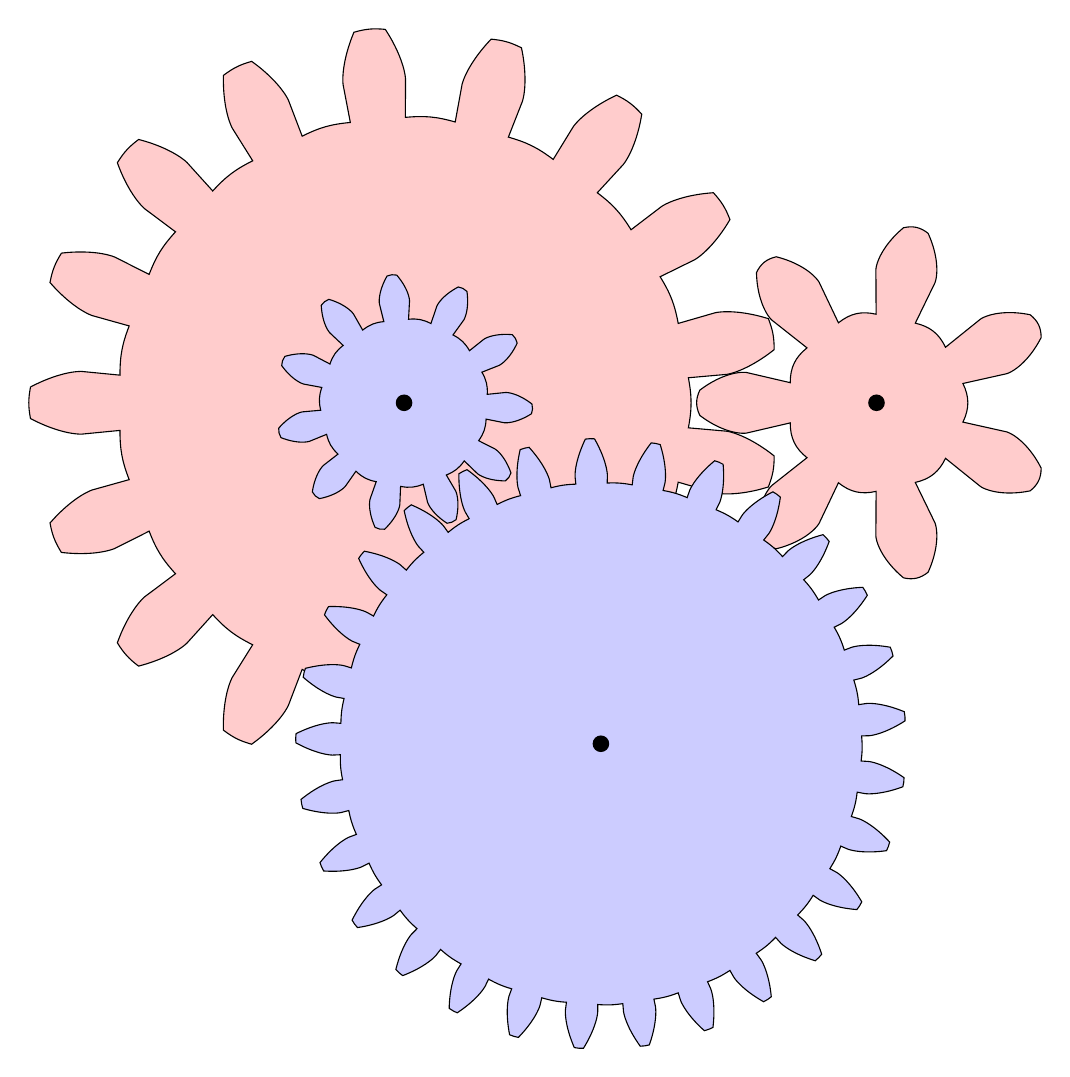
\begin{tikzpicture}
    % observations:
    %
    %  - param #1 and #3 must be equal for gears to mesh
    %  - the required distance is (#2_1 + #2_2) * #1 / 2
    %  - for odd numbers of teeth, gears on a horizontal axis fit without rotation

    \pic[draw,fill=red!20!white]                     at (0,0)   {gear={0.50}{17}{15}};
    \pic[draw,fill=red!20!white]                     at (6,0)   {gear={0.50}{ 7}{15}};

    \pic[draw,fill=blue!20!white,rotate=-60 + 90/11] at (0,0)   {gear={0.25}{11}{20}};
    \pic[draw,fill=blue!20!white,rotate=-60 - 90/29] at (-60:5) {gear={0.25}{29}{20}};

    \foreach \p in {(0,0),(6,0),(-60:5)} \fill \p circle (3pt);
\end{tikzpicture}
\end{document}